% Created by tikzDevice version 0.12.6 on 2026-07-09 15:42:25
% !TEX encoding = UTF-8 Unicode
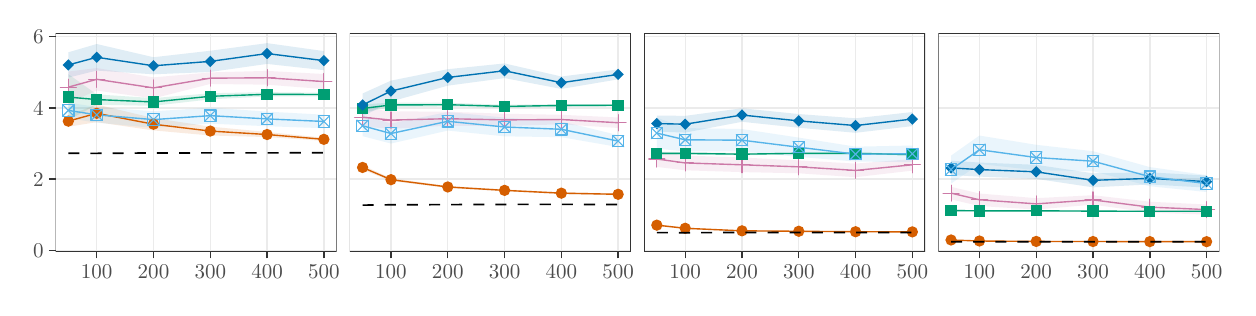
\begin{tikzpicture}[x=1pt,y=1pt]
\definecolor{fillColor}{RGB}{255,255,255}
\path[use as bounding box,fill=fillColor,fill opacity=0.00] (0,0) rectangle (433.62, 93.95);
\begin{scope}
\path[clip] (  0.00,  0.00) rectangle (433.62, 93.95);
\definecolor{drawColor}{RGB}{255,255,255}
\definecolor{fillColor}{RGB}{255,255,255}

\path[draw=drawColor,line width= 0.5pt,line join=round,line cap=round,fill=fillColor] ( -0.00,  0.00) rectangle (433.62, 93.95);
\end{scope}
\begin{scope}
\path[clip] ( 10.07, 12.99) rectangle (111.65, 91.95);
\definecolor{fillColor}{RGB}{255,255,255}

\path[fill=fillColor] ( 10.07, 12.99) rectangle (111.65, 91.95);
\definecolor{drawColor}{gray}{0.92}

\path[draw=drawColor,line width= 0.5pt,line join=round] ( 10.07, 13.41) --
	(111.65, 13.41);

\path[draw=drawColor,line width= 0.5pt,line join=round] ( 10.07, 39.20) --
	(111.65, 39.20);

\path[draw=drawColor,line width= 0.5pt,line join=round] ( 10.07, 64.98) --
	(111.65, 64.98);

\path[draw=drawColor,line width= 0.5pt,line join=round] ( 10.07, 90.77) --
	(111.65, 90.77);

\path[draw=drawColor,line width= 0.5pt,line join=round] ( 24.95, 12.99) --
	( 24.95, 91.95);

\path[draw=drawColor,line width= 0.5pt,line join=round] ( 45.47, 12.99) --
	( 45.47, 91.95);

\path[draw=drawColor,line width= 0.5pt,line join=round] ( 65.99, 12.99) --
	( 65.99, 91.95);

\path[draw=drawColor,line width= 0.5pt,line join=round] ( 86.51, 12.99) --
	( 86.51, 91.95);

\path[draw=drawColor,line width= 0.5pt,line join=round] (107.03, 12.99) --
	(107.03, 91.95);
\definecolor{fillColor}{RGB}{213,94,0}

\path[fill=fillColor,fill opacity=0.12] ( 14.69, 62.21) --
	( 24.95, 66.19) --
	( 45.47, 61.29) --
	( 65.99, 58.19) --
	( 86.51, 56.26) --
	(107.03, 54.17) --
	(107.03, 53.03) --
	( 86.51, 54.42) --
	( 65.99, 54.99) --
	( 45.47, 56.82) --
	( 24.95, 59.82) --
	( 14.69, 58.14) --
	cycle;

\path[] ( 14.69, 62.21) --
	( 24.95, 66.19) --
	( 45.47, 61.29) --
	( 65.99, 58.19) --
	( 86.51, 56.26) --
	(107.03, 54.17);

\path[] (107.03, 53.03) --
	( 86.51, 54.42) --
	( 65.99, 54.99) --
	( 45.47, 56.82) --
	( 24.95, 59.82) --
	( 14.69, 58.14);
\definecolor{fillColor}{RGB}{0,158,115}

\path[fill=fillColor,fill opacity=0.12] ( 14.69, 77.17) --
	( 24.95, 69.84) --
	( 45.47, 68.49) --
	( 65.99, 70.26) --
	( 86.51, 70.66) --
	(107.03, 70.43) --
	(107.03, 69.15) --
	( 86.51, 69.10) --
	( 65.99, 68.05) --
	( 45.47, 65.72) --
	( 24.95, 66.10) --
	( 14.69, 60.57) --
	cycle;

\path[] ( 14.69, 77.17) --
	( 24.95, 69.84) --
	( 45.47, 68.49) --
	( 65.99, 70.26) --
	( 86.51, 70.66) --
	(107.03, 70.43);

\path[] (107.03, 69.15) --
	( 86.51, 69.10) --
	( 65.99, 68.05) --
	( 45.47, 65.72) --
	( 24.95, 66.10) --
	( 14.69, 60.57);
\definecolor{fillColor}{RGB}{0,114,178}

\path[fill=fillColor,fill opacity=0.12] ( 14.69, 85.05) --
	( 24.95, 88.05) --
	( 45.47, 83.27) --
	( 65.99, 85.61) --
	( 86.51, 88.36) --
	(107.03, 85.49) --
	(107.03, 78.60) --
	( 86.51, 80.85) --
	( 65.99, 77.94) --
	( 45.47, 77.10) --
	( 24.95, 78.44) --
	( 14.69, 75.91) --
	cycle;

\path[] ( 14.69, 85.05) --
	( 24.95, 88.05) --
	( 45.47, 83.27) --
	( 65.99, 85.61) --
	( 86.51, 88.36) --
	(107.03, 85.49);

\path[] (107.03, 78.60) --
	( 86.51, 80.85) --
	( 65.99, 77.94) --
	( 45.47, 77.10) --
	( 24.95, 78.44) --
	( 14.69, 75.91);
\definecolor{fillColor}{RGB}{204,121,167}

\path[fill=fillColor,fill opacity=0.12] ( 14.69, 78.10) --
	( 24.95, 79.35) --
	( 45.47, 75.99) --
	( 65.99, 77.79) --
	( 86.51, 78.33) --
	(107.03, 77.20) --
	(107.03, 71.77) --
	( 86.51, 73.35) --
	( 65.99, 73.61) --
	( 45.47, 68.39) --
	( 24.95, 71.22) --
	( 14.69, 66.82) --
	cycle;

\path[] ( 14.69, 78.10) --
	( 24.95, 79.35) --
	( 45.47, 75.99) --
	( 65.99, 77.79) --
	( 86.51, 78.33) --
	(107.03, 77.20);

\path[] (107.03, 71.77) --
	( 86.51, 73.35) --
	( 65.99, 73.61) --
	( 45.47, 68.39) --
	( 24.95, 71.22) --
	( 14.69, 66.82);
\definecolor{fillColor}{RGB}{86,180,233}

\path[fill=fillColor,fill opacity=0.12] ( 14.69, 66.85) --
	( 24.95, 65.29) --
	( 45.47, 63.73) --
	( 65.99, 65.05) --
	( 86.51, 63.62) --
	(107.03, 62.50) --
	(107.03, 57.62) --
	( 86.51, 58.34) --
	( 65.99, 59.28) --
	( 45.47, 57.73) --
	( 24.95, 59.62) --
	( 14.69, 61.24) --
	cycle;

\path[] ( 14.69, 66.85) --
	( 24.95, 65.29) --
	( 45.47, 63.73) --
	( 65.99, 65.05) --
	( 86.51, 63.62) --
	(107.03, 62.50);

\path[] (107.03, 57.62) --
	( 86.51, 58.34) --
	( 65.99, 59.28) --
	( 45.47, 57.73) --
	( 24.95, 59.62) --
	( 14.69, 61.24);
\definecolor{drawColor}{RGB}{213,94,0}

\path[draw=drawColor,line width= 0.5pt,line join=round] ( 14.69, 60.17) --
	( 24.95, 63.01) --
	( 45.47, 59.06) --
	( 65.99, 56.59) --
	( 86.51, 55.34) --
	(107.03, 53.60);
\definecolor{drawColor}{RGB}{0,158,115}

\path[draw=drawColor,line width= 0.5pt,line join=round] ( 14.69, 68.87) --
	( 24.95, 67.97) --
	( 45.47, 67.11) --
	( 65.99, 69.15) --
	( 86.51, 69.88) --
	(107.03, 69.79);
\definecolor{drawColor}{RGB}{0,114,178}

\path[draw=drawColor,line width= 0.5pt,line join=round] ( 14.69, 80.48) --
	( 24.95, 83.25) --
	( 45.47, 80.18) --
	( 65.99, 81.77) --
	( 86.51, 84.60) --
	(107.03, 82.04);
\definecolor{drawColor}{RGB}{204,121,167}

\path[draw=drawColor,line width= 0.5pt,line join=round] ( 14.69, 72.46) --
	( 24.95, 75.29) --
	( 45.47, 72.19) --
	( 65.99, 75.70) --
	( 86.51, 75.84) --
	(107.03, 74.48);
\definecolor{drawColor}{RGB}{86,180,233}

\path[draw=drawColor,line width= 0.5pt,line join=round] ( 14.69, 64.05) --
	( 24.95, 62.45) --
	( 45.47, 60.73) --
	( 65.99, 62.16) --
	( 86.51, 60.98) --
	(107.03, 60.06);
\definecolor{fillColor}{RGB}{213,94,0}

\path[fill=fillColor] ( 14.69, 60.17) circle (  2.05);
\definecolor{drawColor}{RGB}{204,121,167}

\path[draw=drawColor,line width= 0.4pt,line join=round,line cap=round] ( 11.79, 72.46) -- ( 17.59, 72.46);

\path[draw=drawColor,line width= 0.4pt,line join=round,line cap=round] ( 14.69, 69.56) -- ( 14.69, 75.36);
\definecolor{fillColor}{RGB}{0,158,115}

\path[fill=fillColor] ( 12.64, 66.82) --
	( 16.74, 66.82) --
	( 16.74, 70.92) --
	( 12.64, 70.92) --
	cycle;
\definecolor{fillColor}{RGB}{0,114,178}

\path[fill=fillColor] ( 12.64, 80.48) --
	( 14.69, 82.53) --
	( 16.74, 80.48) --
	( 14.69, 78.43) --
	cycle;
\definecolor{drawColor}{RGB}{86,180,233}

\path[draw=drawColor,line width= 0.4pt,line join=round,line cap=round] ( 12.64, 61.99) rectangle ( 16.74, 66.10);

\path[draw=drawColor,line width= 0.4pt,line join=round,line cap=round] ( 12.64, 61.99) -- ( 16.74, 66.10);

\path[draw=drawColor,line width= 0.4pt,line join=round,line cap=round] ( 12.64, 66.10) -- ( 16.74, 61.99);
\definecolor{fillColor}{RGB}{213,94,0}

\path[fill=fillColor] ( 24.95, 63.01) circle (  2.05);
\definecolor{drawColor}{RGB}{204,121,167}

\path[draw=drawColor,line width= 0.4pt,line join=round,line cap=round] ( 22.05, 75.29) -- ( 27.85, 75.29);

\path[draw=drawColor,line width= 0.4pt,line join=round,line cap=round] ( 24.95, 72.39) -- ( 24.95, 78.19);
\definecolor{fillColor}{RGB}{0,158,115}

\path[fill=fillColor] ( 22.90, 65.92) --
	( 27.00, 65.92) --
	( 27.00, 70.02) --
	( 22.90, 70.02) --
	cycle;
\definecolor{fillColor}{RGB}{0,114,178}

\path[fill=fillColor] ( 22.90, 83.25) --
	( 24.95, 85.30) --
	( 27.00, 83.25) --
	( 24.95, 81.20) --
	cycle;
\definecolor{drawColor}{RGB}{86,180,233}

\path[draw=drawColor,line width= 0.4pt,line join=round,line cap=round] ( 22.90, 60.40) rectangle ( 27.00, 64.50);

\path[draw=drawColor,line width= 0.4pt,line join=round,line cap=round] ( 22.90, 60.40) -- ( 27.00, 64.50);

\path[draw=drawColor,line width= 0.4pt,line join=round,line cap=round] ( 22.90, 64.50) -- ( 27.00, 60.40);
\definecolor{fillColor}{RGB}{213,94,0}

\path[fill=fillColor] ( 45.47, 59.06) circle (  2.05);
\definecolor{drawColor}{RGB}{204,121,167}

\path[draw=drawColor,line width= 0.4pt,line join=round,line cap=round] ( 42.57, 72.19) -- ( 48.37, 72.19);

\path[draw=drawColor,line width= 0.4pt,line join=round,line cap=round] ( 45.47, 69.29) -- ( 45.47, 75.09);
\definecolor{fillColor}{RGB}{0,158,115}

\path[fill=fillColor] ( 43.42, 65.06) --
	( 47.52, 65.06) --
	( 47.52, 69.16) --
	( 43.42, 69.16) --
	cycle;
\definecolor{fillColor}{RGB}{0,114,178}

\path[fill=fillColor] ( 43.42, 80.18) --
	( 45.47, 82.24) --
	( 47.52, 80.18) --
	( 45.47, 78.13) --
	cycle;
\definecolor{drawColor}{RGB}{86,180,233}

\path[draw=drawColor,line width= 0.4pt,line join=round,line cap=round] ( 43.42, 58.68) rectangle ( 47.52, 62.78);

\path[draw=drawColor,line width= 0.4pt,line join=round,line cap=round] ( 43.42, 58.68) -- ( 47.52, 62.78);

\path[draw=drawColor,line width= 0.4pt,line join=round,line cap=round] ( 43.42, 62.78) -- ( 47.52, 58.68);
\definecolor{fillColor}{RGB}{213,94,0}

\path[fill=fillColor] ( 65.99, 56.59) circle (  2.05);
\definecolor{drawColor}{RGB}{204,121,167}

\path[draw=drawColor,line width= 0.4pt,line join=round,line cap=round] ( 63.09, 75.70) -- ( 68.89, 75.70);

\path[draw=drawColor,line width= 0.4pt,line join=round,line cap=round] ( 65.99, 72.80) -- ( 65.99, 78.60);
\definecolor{fillColor}{RGB}{0,158,115}

\path[fill=fillColor] ( 63.94, 67.10) --
	( 68.04, 67.10) --
	( 68.04, 71.20) --
	( 63.94, 71.20) --
	cycle;
\definecolor{fillColor}{RGB}{0,114,178}

\path[fill=fillColor] ( 63.94, 81.77) --
	( 65.99, 83.82) --
	( 68.04, 81.77) --
	( 65.99, 79.72) --
	cycle;
\definecolor{drawColor}{RGB}{86,180,233}

\path[draw=drawColor,line width= 0.4pt,line join=round,line cap=round] ( 63.94, 60.11) rectangle ( 68.04, 64.21);

\path[draw=drawColor,line width= 0.4pt,line join=round,line cap=round] ( 63.94, 60.11) -- ( 68.04, 64.21);

\path[draw=drawColor,line width= 0.4pt,line join=round,line cap=round] ( 63.94, 64.21) -- ( 68.04, 60.11);
\definecolor{fillColor}{RGB}{213,94,0}

\path[fill=fillColor] ( 86.51, 55.34) circle (  2.05);
\definecolor{drawColor}{RGB}{204,121,167}

\path[draw=drawColor,line width= 0.4pt,line join=round,line cap=round] ( 83.61, 75.84) -- ( 89.41, 75.84);

\path[draw=drawColor,line width= 0.4pt,line join=round,line cap=round] ( 86.51, 72.94) -- ( 86.51, 78.74);
\definecolor{fillColor}{RGB}{0,158,115}

\path[fill=fillColor] ( 84.46, 67.83) --
	( 88.56, 67.83) --
	( 88.56, 71.93) --
	( 84.46, 71.93) --
	cycle;
\definecolor{fillColor}{RGB}{0,114,178}

\path[fill=fillColor] ( 84.46, 84.60) --
	( 86.51, 86.66) --
	( 88.56, 84.60) --
	( 86.51, 82.55) --
	cycle;
\definecolor{drawColor}{RGB}{86,180,233}

\path[draw=drawColor,line width= 0.4pt,line join=round,line cap=round] ( 84.46, 58.93) rectangle ( 88.56, 63.03);

\path[draw=drawColor,line width= 0.4pt,line join=round,line cap=round] ( 84.46, 58.93) -- ( 88.56, 63.03);

\path[draw=drawColor,line width= 0.4pt,line join=round,line cap=round] ( 84.46, 63.03) -- ( 88.56, 58.93);
\definecolor{fillColor}{RGB}{213,94,0}

\path[fill=fillColor] (107.03, 53.60) circle (  2.05);
\definecolor{drawColor}{RGB}{204,121,167}

\path[draw=drawColor,line width= 0.4pt,line join=round,line cap=round] (104.13, 74.48) -- (109.93, 74.48);

\path[draw=drawColor,line width= 0.4pt,line join=round,line cap=round] (107.03, 71.58) -- (107.03, 77.38);
\definecolor{fillColor}{RGB}{0,158,115}

\path[fill=fillColor] (104.98, 67.74) --
	(109.08, 67.74) --
	(109.08, 71.84) --
	(104.98, 71.84) --
	cycle;
\definecolor{fillColor}{RGB}{0,114,178}

\path[fill=fillColor] (104.98, 82.04) --
	(107.03, 84.09) --
	(109.08, 82.04) --
	(107.03, 79.99) --
	cycle;
\definecolor{drawColor}{RGB}{86,180,233}

\path[draw=drawColor,line width= 0.4pt,line join=round,line cap=round] (104.98, 58.01) rectangle (109.08, 62.11);

\path[draw=drawColor,line width= 0.4pt,line join=round,line cap=round] (104.98, 58.01) -- (109.08, 62.11);

\path[draw=drawColor,line width= 0.4pt,line join=round,line cap=round] (104.98, 62.11) -- (109.08, 58.01);
\definecolor{drawColor}{RGB}{0,0,0}

\path[draw=drawColor,line width= 0.6pt,dash pattern=on 4pt off 4pt ,line join=round] ( 14.69, 48.55) --
	( 24.95, 48.54) --
	( 45.47, 48.67) --
	( 65.99, 48.70) --
	( 86.51, 48.71) --
	(107.03, 48.77);
\definecolor{drawColor}{gray}{0.20}

\path[draw=drawColor,line width= 0.5pt,line join=round,line cap=round] ( 10.07, 12.99) rectangle (111.65, 91.95);
\end{scope}
\begin{scope}
\path[clip] (116.40, 12.99) rectangle (217.97, 91.95);
\definecolor{fillColor}{RGB}{255,255,255}

\path[fill=fillColor] (116.40, 12.99) rectangle (217.97, 91.95);
\definecolor{drawColor}{gray}{0.92}

\path[draw=drawColor,line width= 0.5pt,line join=round] (116.40, 13.41) --
	(217.97, 13.41);

\path[draw=drawColor,line width= 0.5pt,line join=round] (116.40, 39.20) --
	(217.97, 39.20);

\path[draw=drawColor,line width= 0.5pt,line join=round] (116.40, 64.98) --
	(217.97, 64.98);

\path[draw=drawColor,line width= 0.5pt,line join=round] (116.40, 90.77) --
	(217.97, 90.77);

\path[draw=drawColor,line width= 0.5pt,line join=round] (131.28, 12.99) --
	(131.28, 91.95);

\path[draw=drawColor,line width= 0.5pt,line join=round] (151.80, 12.99) --
	(151.80, 91.95);

\path[draw=drawColor,line width= 0.5pt,line join=round] (172.32, 12.99) --
	(172.32, 91.95);

\path[draw=drawColor,line width= 0.5pt,line join=round] (192.84, 12.99) --
	(192.84, 91.95);

\path[draw=drawColor,line width= 0.5pt,line join=round] (213.36, 12.99) --
	(213.36, 91.95);
\definecolor{fillColor}{RGB}{213,94,0}

\path[fill=fillColor,fill opacity=0.12] (121.02, 44.26) --
	(131.28, 39.52) --
	(151.80, 36.78) --
	(172.32, 35.52) --
	(192.84, 34.50) --
	(213.36, 34.10) --
	(213.36, 33.38) --
	(192.84, 33.80) --
	(172.32, 34.80) --
	(151.80, 36.00) --
	(131.28, 38.52) --
	(121.02, 42.62) --
	cycle;

\path[] (121.02, 44.26) --
	(131.28, 39.52) --
	(151.80, 36.78) --
	(172.32, 35.52) --
	(192.84, 34.50) --
	(213.36, 34.10);

\path[] (213.36, 33.38) --
	(192.84, 33.80) --
	(172.32, 34.80) --
	(151.80, 36.00) --
	(131.28, 38.52) --
	(121.02, 42.62);
\definecolor{fillColor}{RGB}{0,158,115}

\path[fill=fillColor,fill opacity=0.12] (121.02, 66.23) --
	(131.28, 66.86) --
	(151.80, 66.82) --
	(172.32, 66.11) --
	(192.84, 66.33) --
	(213.36, 66.29) --
	(213.36, 65.53) --
	(192.84, 65.34) --
	(172.32, 64.90) --
	(151.80, 65.42) --
	(131.28, 65.18) --
	(121.02, 63.28) --
	cycle;

\path[] (121.02, 66.23) --
	(131.28, 66.86) --
	(151.80, 66.82) --
	(172.32, 66.11) --
	(192.84, 66.33) --
	(213.36, 66.29);

\path[] (213.36, 65.53) --
	(192.84, 65.34) --
	(172.32, 64.90) --
	(151.80, 65.42) --
	(131.28, 65.18) --
	(121.02, 63.28);
\definecolor{fillColor}{RGB}{0,114,178}

\path[fill=fillColor,fill opacity=0.12] (121.02, 70.17) --
	(131.28, 74.81) --
	(151.80, 78.94) --
	(172.32, 81.03) --
	(192.84, 76.31) --
	(213.36, 78.85) --
	(213.36, 75.28) --
	(192.84, 71.81) --
	(172.32, 75.73) --
	(151.80, 72.99) --
	(131.28, 67.27) --
	(121.02, 61.85) --
	cycle;

\path[] (121.02, 70.17) --
	(131.28, 74.81) --
	(151.80, 78.94) --
	(172.32, 81.03) --
	(192.84, 76.31) --
	(213.36, 78.85);

\path[] (213.36, 75.28) --
	(192.84, 71.81) --
	(172.32, 75.73) --
	(151.80, 72.99) --
	(131.28, 67.27) --
	(121.02, 61.85);
\definecolor{fillColor}{RGB}{204,121,167}

\path[fill=fillColor,fill opacity=0.12] (121.02, 64.94) --
	(131.28, 63.74) --
	(151.80, 63.57) --
	(172.32, 62.85) --
	(192.84, 62.47) --
	(213.36, 61.50) --
	(213.36, 57.71) --
	(192.84, 59.03) --
	(172.32, 58.40) --
	(151.80, 58.52) --
	(131.28, 57.39) --
	(121.02, 58.22) --
	cycle;

\path[] (121.02, 64.94) --
	(131.28, 63.74) --
	(151.80, 63.57) --
	(172.32, 62.85) --
	(192.84, 62.47) --
	(213.36, 61.50);

\path[] (213.36, 57.71) --
	(192.84, 59.03) --
	(172.32, 58.40) --
	(151.80, 58.52) --
	(131.28, 57.39) --
	(121.02, 58.22);
\definecolor{fillColor}{RGB}{86,180,233}

\path[fill=fillColor,fill opacity=0.12] (121.02, 62.24) --
	(131.28, 59.33) --
	(151.80, 63.47) --
	(172.32, 61.45) --
	(192.84, 60.09) --
	(213.36, 55.12) --
	(213.36, 50.83) --
	(192.84, 54.38) --
	(172.32, 54.68) --
	(151.80, 56.77) --
	(131.28, 52.08) --
	(121.02, 54.75) --
	cycle;

\path[] (121.02, 62.24) --
	(131.28, 59.33) --
	(151.80, 63.47) --
	(172.32, 61.45) --
	(192.84, 60.09) --
	(213.36, 55.12);

\path[] (213.36, 50.83) --
	(192.84, 54.38) --
	(172.32, 54.68) --
	(151.80, 56.77) --
	(131.28, 52.08) --
	(121.02, 54.75);
\definecolor{drawColor}{RGB}{213,94,0}

\path[draw=drawColor,line width= 0.5pt,line join=round] (121.02, 43.44) --
	(131.28, 39.02) --
	(151.80, 36.39) --
	(172.32, 35.16) --
	(192.84, 34.15) --
	(213.36, 33.74);
\definecolor{drawColor}{RGB}{0,158,115}

\path[draw=drawColor,line width= 0.5pt,line join=round] (121.02, 64.75) --
	(131.28, 66.02) --
	(151.80, 66.12) --
	(172.32, 65.50) --
	(192.84, 65.84) --
	(213.36, 65.91);
\definecolor{drawColor}{RGB}{0,114,178}

\path[draw=drawColor,line width= 0.5pt,line join=round] (121.02, 66.01) --
	(131.28, 71.04) --
	(151.80, 75.96) --
	(172.32, 78.38) --
	(192.84, 74.06) --
	(213.36, 77.06);
\definecolor{drawColor}{RGB}{204,121,167}

\path[draw=drawColor,line width= 0.5pt,line join=round] (121.02, 61.58) --
	(131.28, 60.56) --
	(151.80, 61.05) --
	(172.32, 60.63) --
	(192.84, 60.75) --
	(213.36, 59.60);
\definecolor{drawColor}{RGB}{86,180,233}

\path[draw=drawColor,line width= 0.5pt,line join=round] (121.02, 58.49) --
	(131.28, 55.70) --
	(151.80, 60.12) --
	(172.32, 58.06) --
	(192.84, 57.23) --
	(213.36, 52.97);
\definecolor{fillColor}{RGB}{213,94,0}

\path[fill=fillColor] (121.02, 43.44) circle (  2.05);
\definecolor{drawColor}{RGB}{204,121,167}

\path[draw=drawColor,line width= 0.4pt,line join=round,line cap=round] (118.11, 61.58) -- (123.92, 61.58);

\path[draw=drawColor,line width= 0.4pt,line join=round,line cap=round] (121.02, 58.68) -- (121.02, 64.48);
\definecolor{fillColor}{RGB}{0,158,115}

\path[fill=fillColor] (118.96, 62.70) --
	(123.07, 62.70) --
	(123.07, 66.80) --
	(118.96, 66.80) --
	cycle;
\definecolor{fillColor}{RGB}{0,114,178}

\path[fill=fillColor] (118.96, 66.01) --
	(121.02, 68.06) --
	(123.07, 66.01) --
	(121.02, 63.96) --
	cycle;
\definecolor{drawColor}{RGB}{86,180,233}

\path[draw=drawColor,line width= 0.4pt,line join=round,line cap=round] (118.96, 56.44) rectangle (123.07, 60.54);

\path[draw=drawColor,line width= 0.4pt,line join=round,line cap=round] (118.96, 56.44) -- (123.07, 60.54);

\path[draw=drawColor,line width= 0.4pt,line join=round,line cap=round] (118.96, 60.54) -- (123.07, 56.44);
\definecolor{fillColor}{RGB}{213,94,0}

\path[fill=fillColor] (131.28, 39.02) circle (  2.05);
\definecolor{drawColor}{RGB}{204,121,167}

\path[draw=drawColor,line width= 0.4pt,line join=round,line cap=round] (128.37, 60.56) -- (134.18, 60.56);

\path[draw=drawColor,line width= 0.4pt,line join=round,line cap=round] (131.28, 57.66) -- (131.28, 63.47);
\definecolor{fillColor}{RGB}{0,158,115}

\path[fill=fillColor] (129.22, 63.97) --
	(133.33, 63.97) --
	(133.33, 68.07) --
	(129.22, 68.07) --
	cycle;
\definecolor{fillColor}{RGB}{0,114,178}

\path[fill=fillColor] (129.22, 71.04) --
	(131.28, 73.09) --
	(133.33, 71.04) --
	(131.28, 68.99) --
	cycle;
\definecolor{drawColor}{RGB}{86,180,233}

\path[draw=drawColor,line width= 0.4pt,line join=round,line cap=round] (129.22, 53.65) rectangle (133.33, 57.75);

\path[draw=drawColor,line width= 0.4pt,line join=round,line cap=round] (129.22, 53.65) -- (133.33, 57.75);

\path[draw=drawColor,line width= 0.4pt,line join=round,line cap=round] (129.22, 57.75) -- (133.33, 53.65);
\definecolor{fillColor}{RGB}{213,94,0}

\path[fill=fillColor] (151.80, 36.39) circle (  2.05);
\definecolor{drawColor}{RGB}{204,121,167}

\path[draw=drawColor,line width= 0.4pt,line join=round,line cap=round] (148.89, 61.05) -- (154.70, 61.05);

\path[draw=drawColor,line width= 0.4pt,line join=round,line cap=round] (151.80, 58.15) -- (151.80, 63.95);
\definecolor{fillColor}{RGB}{0,158,115}

\path[fill=fillColor] (149.74, 64.07) --
	(153.85, 64.07) --
	(153.85, 68.17) --
	(149.74, 68.17) --
	cycle;
\definecolor{fillColor}{RGB}{0,114,178}

\path[fill=fillColor] (149.74, 75.96) --
	(151.80, 78.02) --
	(153.85, 75.96) --
	(151.80, 73.91) --
	cycle;
\definecolor{drawColor}{RGB}{86,180,233}

\path[draw=drawColor,line width= 0.4pt,line join=round,line cap=round] (149.74, 58.07) rectangle (153.85, 62.17);

\path[draw=drawColor,line width= 0.4pt,line join=round,line cap=round] (149.74, 58.07) -- (153.85, 62.17);

\path[draw=drawColor,line width= 0.4pt,line join=round,line cap=round] (149.74, 62.17) -- (153.85, 58.07);
\definecolor{fillColor}{RGB}{213,94,0}

\path[fill=fillColor] (172.32, 35.16) circle (  2.05);
\definecolor{drawColor}{RGB}{204,121,167}

\path[draw=drawColor,line width= 0.4pt,line join=round,line cap=round] (169.41, 60.63) -- (175.22, 60.63);

\path[draw=drawColor,line width= 0.4pt,line join=round,line cap=round] (172.32, 57.73) -- (172.32, 63.53);
\definecolor{fillColor}{RGB}{0,158,115}

\path[fill=fillColor] (170.26, 63.45) --
	(174.37, 63.45) --
	(174.37, 67.55) --
	(170.26, 67.55) --
	cycle;
\definecolor{fillColor}{RGB}{0,114,178}

\path[fill=fillColor] (170.26, 78.38) --
	(172.32, 80.43) --
	(174.37, 78.38) --
	(172.32, 76.33) --
	cycle;
\definecolor{drawColor}{RGB}{86,180,233}

\path[draw=drawColor,line width= 0.4pt,line join=round,line cap=round] (170.26, 56.01) rectangle (174.37, 60.12);

\path[draw=drawColor,line width= 0.4pt,line join=round,line cap=round] (170.26, 56.01) -- (174.37, 60.12);

\path[draw=drawColor,line width= 0.4pt,line join=round,line cap=round] (170.26, 60.12) -- (174.37, 56.01);
\definecolor{fillColor}{RGB}{213,94,0}

\path[fill=fillColor] (192.84, 34.15) circle (  2.05);
\definecolor{drawColor}{RGB}{204,121,167}

\path[draw=drawColor,line width= 0.4pt,line join=round,line cap=round] (189.93, 60.75) -- (195.74, 60.75);

\path[draw=drawColor,line width= 0.4pt,line join=round,line cap=round] (192.84, 57.85) -- (192.84, 63.65);
\definecolor{fillColor}{RGB}{0,158,115}

\path[fill=fillColor] (190.78, 63.79) --
	(194.89, 63.79) --
	(194.89, 67.89) --
	(190.78, 67.89) --
	cycle;
\definecolor{fillColor}{RGB}{0,114,178}

\path[fill=fillColor] (190.78, 74.06) --
	(192.84, 76.11) --
	(194.89, 74.06) --
	(192.84, 72.01) --
	cycle;
\definecolor{drawColor}{RGB}{86,180,233}

\path[draw=drawColor,line width= 0.4pt,line join=round,line cap=round] (190.78, 55.18) rectangle (194.89, 59.28);

\path[draw=drawColor,line width= 0.4pt,line join=round,line cap=round] (190.78, 55.18) -- (194.89, 59.28);

\path[draw=drawColor,line width= 0.4pt,line join=round,line cap=round] (190.78, 59.28) -- (194.89, 55.18);
\definecolor{fillColor}{RGB}{213,94,0}

\path[fill=fillColor] (213.36, 33.74) circle (  2.05);
\definecolor{drawColor}{RGB}{204,121,167}

\path[draw=drawColor,line width= 0.4pt,line join=round,line cap=round] (210.45, 59.60) -- (216.26, 59.60);

\path[draw=drawColor,line width= 0.4pt,line join=round,line cap=round] (213.36, 56.70) -- (213.36, 62.51);
\definecolor{fillColor}{RGB}{0,158,115}

\path[fill=fillColor] (211.30, 63.86) --
	(215.41, 63.86) --
	(215.41, 67.96) --
	(211.30, 67.96) --
	cycle;
\definecolor{fillColor}{RGB}{0,114,178}

\path[fill=fillColor] (211.30, 77.06) --
	(213.36, 79.11) --
	(215.41, 77.06) --
	(213.36, 75.01) --
	cycle;
\definecolor{drawColor}{RGB}{86,180,233}

\path[draw=drawColor,line width= 0.4pt,line join=round,line cap=round] (211.30, 50.92) rectangle (215.41, 55.02);

\path[draw=drawColor,line width= 0.4pt,line join=round,line cap=round] (211.30, 50.92) -- (215.41, 55.02);

\path[draw=drawColor,line width= 0.4pt,line join=round,line cap=round] (211.30, 55.02) -- (215.41, 50.92);
\definecolor{drawColor}{RGB}{0,0,0}

\path[draw=drawColor,line width= 0.6pt,dash pattern=on 4pt off 4pt ,line join=round] (121.02, 29.82) --
	(131.28, 29.95) --
	(151.80, 30.01) --
	(172.32, 30.08) --
	(192.84, 30.10) --
	(213.36, 30.05);
\definecolor{drawColor}{gray}{0.20}

\path[draw=drawColor,line width= 0.5pt,line join=round,line cap=round] (116.40, 12.99) rectangle (217.97, 91.95);
\end{scope}
\begin{scope}
\path[clip] (222.72, 12.99) rectangle (324.30, 91.95);
\definecolor{fillColor}{RGB}{255,255,255}

\path[fill=fillColor] (222.72, 12.99) rectangle (324.30, 91.95);
\definecolor{drawColor}{gray}{0.92}

\path[draw=drawColor,line width= 0.5pt,line join=round] (222.72, 13.41) --
	(324.30, 13.41);

\path[draw=drawColor,line width= 0.5pt,line join=round] (222.72, 39.20) --
	(324.30, 39.20);

\path[draw=drawColor,line width= 0.5pt,line join=round] (222.72, 64.98) --
	(324.30, 64.98);

\path[draw=drawColor,line width= 0.5pt,line join=round] (222.72, 90.77) --
	(324.30, 90.77);

\path[draw=drawColor,line width= 0.5pt,line join=round] (237.60, 12.99) --
	(237.60, 91.95);

\path[draw=drawColor,line width= 0.5pt,line join=round] (258.12, 12.99) --
	(258.12, 91.95);

\path[draw=drawColor,line width= 0.5pt,line join=round] (278.64, 12.99) --
	(278.64, 91.95);

\path[draw=drawColor,line width= 0.5pt,line join=round] (299.16, 12.99) --
	(299.16, 91.95);

\path[draw=drawColor,line width= 0.5pt,line join=round] (319.68, 12.99) --
	(319.68, 91.95);
\definecolor{fillColor}{RGB}{213,94,0}

\path[fill=fillColor,fill opacity=0.12] (227.34, 22.89) --
	(237.60, 21.73) --
	(258.12, 20.62) --
	(278.64, 20.52) --
	(299.16, 20.26) --
	(319.68, 20.21) --
	(319.68, 20.11) --
	(299.16, 20.16) --
	(278.64, 20.24) --
	(258.12, 20.46) --
	(237.60, 21.18) --
	(227.34, 22.29) --
	cycle;

\path[] (227.34, 22.89) --
	(237.60, 21.73) --
	(258.12, 20.62) --
	(278.64, 20.52) --
	(299.16, 20.26) --
	(319.68, 20.21);

\path[] (319.68, 20.11) --
	(299.16, 20.16) --
	(278.64, 20.24) --
	(258.12, 20.46) --
	(237.60, 21.18) --
	(227.34, 22.29);
\definecolor{fillColor}{RGB}{0,158,115}

\path[fill=fillColor,fill opacity=0.12] (227.34, 49.14) --
	(237.60, 48.99) --
	(258.12, 48.66) --
	(278.64, 48.84) --
	(299.16, 48.83) --
	(319.68, 48.42) --
	(319.68, 47.69) --
	(299.16, 48.26) --
	(278.64, 48.24) --
	(258.12, 47.82) --
	(237.60, 48.05) --
	(227.34, 47.89) --
	cycle;

\path[] (227.34, 49.14) --
	(237.60, 48.99) --
	(258.12, 48.66) --
	(278.64, 48.84) --
	(299.16, 48.83) --
	(319.68, 48.42);

\path[] (319.68, 47.69) --
	(299.16, 48.26) --
	(278.64, 48.24) --
	(258.12, 47.82) --
	(237.60, 48.05) --
	(227.34, 47.89);
\definecolor{fillColor}{RGB}{0,114,178}

\path[fill=fillColor,fill opacity=0.12] (227.34, 62.19) --
	(237.60, 62.09) --
	(258.12, 64.82) --
	(278.64, 62.74) --
	(299.16, 61.20) --
	(319.68, 63.46) --
	(319.68, 58.39) --
	(299.16, 55.96) --
	(278.64, 57.79) --
	(258.12, 59.94) --
	(237.60, 56.04) --
	(227.34, 56.40) --
	cycle;

\path[] (227.34, 62.19) --
	(237.60, 62.09) --
	(258.12, 64.82) --
	(278.64, 62.74) --
	(299.16, 61.20) --
	(319.68, 63.46);

\path[] (319.68, 58.39) --
	(299.16, 55.96) --
	(278.64, 57.79) --
	(258.12, 59.94) --
	(237.60, 56.04) --
	(227.34, 56.40);
\definecolor{fillColor}{RGB}{204,121,167}

\path[fill=fillColor,fill opacity=0.12] (227.34, 49.34) --
	(237.60, 47.73) --
	(258.12, 47.04) --
	(278.64, 45.99) --
	(299.16, 44.83) --
	(319.68, 46.49) --
	(319.68, 42.30) --
	(299.16, 39.92) --
	(278.64, 41.33) --
	(258.12, 41.76) --
	(237.60, 42.41) --
	(227.34, 43.63) --
	cycle;

\path[] (227.34, 49.34) --
	(237.60, 47.73) --
	(258.12, 47.04) --
	(278.64, 45.99) --
	(299.16, 44.83) --
	(319.68, 46.49);

\path[] (319.68, 42.30) --
	(299.16, 39.92) --
	(278.64, 41.33) --
	(258.12, 41.76) --
	(237.60, 42.41) --
	(227.34, 43.63);
\definecolor{fillColor}{RGB}{86,180,233}

\path[fill=fillColor,fill opacity=0.12] (227.34, 61.42) --
	(237.60, 57.67) --
	(258.12, 57.32) --
	(278.64, 54.22) --
	(299.16, 50.95) --
	(319.68, 51.36) --
	(319.68, 45.36) --
	(299.16, 45.56) --
	(278.64, 47.27) --
	(258.12, 49.27) --
	(237.60, 49.20) --
	(227.34, 50.28) --
	cycle;

\path[] (227.34, 61.42) --
	(237.60, 57.67) --
	(258.12, 57.32) --
	(278.64, 54.22) --
	(299.16, 50.95) --
	(319.68, 51.36);

\path[] (319.68, 45.36) --
	(299.16, 45.56) --
	(278.64, 47.27) --
	(258.12, 49.27) --
	(237.60, 49.20) --
	(227.34, 50.28);
\definecolor{drawColor}{RGB}{213,94,0}

\path[draw=drawColor,line width= 0.5pt,line join=round] (227.34, 22.59) --
	(237.60, 21.46) --
	(258.12, 20.54) --
	(278.64, 20.38) --
	(299.16, 20.21) --
	(319.68, 20.16);
\definecolor{drawColor}{RGB}{0,158,115}

\path[draw=drawColor,line width= 0.5pt,line join=round] (227.34, 48.51) --
	(237.60, 48.52) --
	(258.12, 48.24) --
	(278.64, 48.54) --
	(299.16, 48.55) --
	(319.68, 48.06);
\definecolor{drawColor}{RGB}{0,114,178}

\path[draw=drawColor,line width= 0.5pt,line join=round] (227.34, 59.29) --
	(237.60, 59.07) --
	(258.12, 62.38) --
	(278.64, 60.27) --
	(299.16, 58.58) --
	(319.68, 60.93);
\definecolor{drawColor}{RGB}{204,121,167}

\path[draw=drawColor,line width= 0.5pt,line join=round] (227.34, 46.49) --
	(237.60, 45.07) --
	(258.12, 44.40) --
	(278.64, 43.66) --
	(299.16, 42.37) --
	(319.68, 44.40);
\definecolor{drawColor}{RGB}{86,180,233}

\path[draw=drawColor,line width= 0.5pt,line join=round] (227.34, 55.85) --
	(237.60, 53.43) --
	(258.12, 53.29) --
	(278.64, 50.74) --
	(299.16, 48.25) --
	(319.68, 48.36);
\definecolor{fillColor}{RGB}{213,94,0}

\path[fill=fillColor] (227.34, 22.59) circle (  2.05);
\definecolor{drawColor}{RGB}{204,121,167}

\path[draw=drawColor,line width= 0.4pt,line join=round,line cap=round] (224.44, 46.49) -- (230.24, 46.49);

\path[draw=drawColor,line width= 0.4pt,line join=round,line cap=round] (227.34, 43.58) -- (227.34, 49.39);
\definecolor{fillColor}{RGB}{0,158,115}

\path[fill=fillColor] (225.29, 46.46) --
	(229.39, 46.46) --
	(229.39, 50.56) --
	(225.29, 50.56) --
	cycle;
\definecolor{fillColor}{RGB}{0,114,178}

\path[fill=fillColor] (225.29, 59.29) --
	(227.34, 61.34) --
	(229.39, 59.29) --
	(227.34, 57.24) --
	cycle;
\definecolor{drawColor}{RGB}{86,180,233}

\path[draw=drawColor,line width= 0.4pt,line join=round,line cap=round] (225.29, 53.80) rectangle (229.39, 57.90);

\path[draw=drawColor,line width= 0.4pt,line join=round,line cap=round] (225.29, 53.80) -- (229.39, 57.90);

\path[draw=drawColor,line width= 0.4pt,line join=round,line cap=round] (225.29, 57.90) -- (229.39, 53.80);
\definecolor{fillColor}{RGB}{213,94,0}

\path[fill=fillColor] (237.60, 21.46) circle (  2.05);
\definecolor{drawColor}{RGB}{204,121,167}

\path[draw=drawColor,line width= 0.4pt,line join=round,line cap=round] (234.70, 45.07) -- (240.50, 45.07);

\path[draw=drawColor,line width= 0.4pt,line join=round,line cap=round] (237.60, 42.17) -- (237.60, 47.97);
\definecolor{fillColor}{RGB}{0,158,115}

\path[fill=fillColor] (235.55, 46.47) --
	(239.65, 46.47) --
	(239.65, 50.57) --
	(235.55, 50.57) --
	cycle;
\definecolor{fillColor}{RGB}{0,114,178}

\path[fill=fillColor] (235.55, 59.07) --
	(237.60, 61.12) --
	(239.65, 59.07) --
	(237.60, 57.02) --
	cycle;
\definecolor{drawColor}{RGB}{86,180,233}

\path[draw=drawColor,line width= 0.4pt,line join=round,line cap=round] (235.55, 51.38) rectangle (239.65, 55.48);

\path[draw=drawColor,line width= 0.4pt,line join=round,line cap=round] (235.55, 51.38) -- (239.65, 55.48);

\path[draw=drawColor,line width= 0.4pt,line join=round,line cap=round] (235.55, 55.48) -- (239.65, 51.38);
\definecolor{fillColor}{RGB}{213,94,0}

\path[fill=fillColor] (258.12, 20.54) circle (  2.05);
\definecolor{drawColor}{RGB}{204,121,167}

\path[draw=drawColor,line width= 0.4pt,line join=round,line cap=round] (255.22, 44.40) -- (261.02, 44.40);

\path[draw=drawColor,line width= 0.4pt,line join=round,line cap=round] (258.12, 41.50) -- (258.12, 47.30);
\definecolor{fillColor}{RGB}{0,158,115}

\path[fill=fillColor] (256.07, 46.19) --
	(260.17, 46.19) --
	(260.17, 50.29) --
	(256.07, 50.29) --
	cycle;
\definecolor{fillColor}{RGB}{0,114,178}

\path[fill=fillColor] (256.07, 62.38) --
	(258.12, 64.43) --
	(260.17, 62.38) --
	(258.12, 60.33) --
	cycle;
\definecolor{drawColor}{RGB}{86,180,233}

\path[draw=drawColor,line width= 0.4pt,line join=round,line cap=round] (256.07, 51.24) rectangle (260.17, 55.35);

\path[draw=drawColor,line width= 0.4pt,line join=round,line cap=round] (256.07, 51.24) -- (260.17, 55.35);

\path[draw=drawColor,line width= 0.4pt,line join=round,line cap=round] (256.07, 55.35) -- (260.17, 51.24);
\definecolor{fillColor}{RGB}{213,94,0}

\path[fill=fillColor] (278.64, 20.38) circle (  2.05);
\definecolor{drawColor}{RGB}{204,121,167}

\path[draw=drawColor,line width= 0.4pt,line join=round,line cap=round] (275.74, 43.66) -- (281.54, 43.66);

\path[draw=drawColor,line width= 0.4pt,line join=round,line cap=round] (278.64, 40.76) -- (278.64, 46.56);
\definecolor{fillColor}{RGB}{0,158,115}

\path[fill=fillColor] (276.59, 46.49) --
	(280.69, 46.49) --
	(280.69, 50.59) --
	(276.59, 50.59) --
	cycle;
\definecolor{fillColor}{RGB}{0,114,178}

\path[fill=fillColor] (276.59, 60.27) --
	(278.64, 62.32) --
	(280.69, 60.27) --
	(278.64, 58.21) --
	cycle;
\definecolor{drawColor}{RGB}{86,180,233}

\path[draw=drawColor,line width= 0.4pt,line join=round,line cap=round] (276.59, 48.69) rectangle (280.69, 52.80);

\path[draw=drawColor,line width= 0.4pt,line join=round,line cap=round] (276.59, 48.69) -- (280.69, 52.80);

\path[draw=drawColor,line width= 0.4pt,line join=round,line cap=round] (276.59, 52.80) -- (280.69, 48.69);
\definecolor{fillColor}{RGB}{213,94,0}

\path[fill=fillColor] (299.16, 20.21) circle (  2.05);
\definecolor{drawColor}{RGB}{204,121,167}

\path[draw=drawColor,line width= 0.4pt,line join=round,line cap=round] (296.26, 42.37) -- (302.06, 42.37);

\path[draw=drawColor,line width= 0.4pt,line join=round,line cap=round] (299.16, 39.47) -- (299.16, 45.27);
\definecolor{fillColor}{RGB}{0,158,115}

\path[fill=fillColor] (297.11, 46.50) --
	(301.21, 46.50) --
	(301.21, 50.60) --
	(297.11, 50.60) --
	cycle;
\definecolor{fillColor}{RGB}{0,114,178}

\path[fill=fillColor] (297.11, 58.58) --
	(299.16, 60.63) --
	(301.21, 58.58) --
	(299.16, 56.53) --
	cycle;
\definecolor{drawColor}{RGB}{86,180,233}

\path[draw=drawColor,line width= 0.4pt,line join=round,line cap=round] (297.11, 46.20) rectangle (301.21, 50.30);

\path[draw=drawColor,line width= 0.4pt,line join=round,line cap=round] (297.11, 46.20) -- (301.21, 50.30);

\path[draw=drawColor,line width= 0.4pt,line join=round,line cap=round] (297.11, 50.30) -- (301.21, 46.20);
\definecolor{fillColor}{RGB}{213,94,0}

\path[fill=fillColor] (319.68, 20.16) circle (  2.05);
\definecolor{drawColor}{RGB}{204,121,167}

\path[draw=drawColor,line width= 0.4pt,line join=round,line cap=round] (316.78, 44.40) -- (322.58, 44.40);

\path[draw=drawColor,line width= 0.4pt,line join=round,line cap=round] (319.68, 41.50) -- (319.68, 47.30);
\definecolor{fillColor}{RGB}{0,158,115}

\path[fill=fillColor] (317.63, 46.00) --
	(321.73, 46.00) --
	(321.73, 50.11) --
	(317.63, 50.11) --
	cycle;
\definecolor{fillColor}{RGB}{0,114,178}

\path[fill=fillColor] (317.63, 60.93) --
	(319.68, 62.98) --
	(321.73, 60.93) --
	(319.68, 58.87) --
	cycle;
\definecolor{drawColor}{RGB}{86,180,233}

\path[draw=drawColor,line width= 0.4pt,line join=round,line cap=round] (317.63, 46.31) rectangle (321.73, 50.41);

\path[draw=drawColor,line width= 0.4pt,line join=round,line cap=round] (317.63, 46.31) -- (321.73, 50.41);

\path[draw=drawColor,line width= 0.4pt,line join=round,line cap=round] (317.63, 50.41) -- (321.73, 46.31);
\definecolor{drawColor}{RGB}{0,0,0}

\path[draw=drawColor,line width= 0.6pt,dash pattern=on 4pt off 4pt ,line join=round] (227.34, 19.90) --
	(237.60, 19.86) --
	(258.12, 19.93) --
	(278.64, 19.93) --
	(299.16, 19.94) --
	(319.68, 19.96);
\definecolor{drawColor}{gray}{0.20}

\path[draw=drawColor,line width= 0.5pt,line join=round,line cap=round] (222.72, 12.99) rectangle (324.30, 91.95);
\end{scope}
\begin{scope}
\path[clip] (329.05, 12.99) rectangle (430.62, 91.95);
\definecolor{fillColor}{RGB}{255,255,255}

\path[fill=fillColor] (329.05, 12.99) rectangle (430.62, 91.95);
\definecolor{drawColor}{gray}{0.92}

\path[draw=drawColor,line width= 0.5pt,line join=round] (329.05, 13.41) --
	(430.62, 13.41);

\path[draw=drawColor,line width= 0.5pt,line join=round] (329.05, 39.20) --
	(430.62, 39.20);

\path[draw=drawColor,line width= 0.5pt,line join=round] (329.05, 64.98) --
	(430.62, 64.98);

\path[draw=drawColor,line width= 0.5pt,line join=round] (329.05, 90.77) --
	(430.62, 90.77);

\path[draw=drawColor,line width= 0.5pt,line join=round] (343.92, 12.99) --
	(343.92, 91.95);

\path[draw=drawColor,line width= 0.5pt,line join=round] (364.44, 12.99) --
	(364.44, 91.95);

\path[draw=drawColor,line width= 0.5pt,line join=round] (384.96, 12.99) --
	(384.96, 91.95);

\path[draw=drawColor,line width= 0.5pt,line join=round] (405.48, 12.99) --
	(405.48, 91.95);

\path[draw=drawColor,line width= 0.5pt,line join=round] (426.00, 12.99) --
	(426.00, 91.95);
\definecolor{fillColor}{RGB}{213,94,0}

\path[fill=fillColor,fill opacity=0.12] (333.66, 17.28) --
	(343.92, 16.88) --
	(364.44, 16.73) --
	(384.96, 16.68) --
	(405.48, 16.65) --
	(426.00, 16.63) --
	(426.00, 16.61) --
	(405.48, 16.63) --
	(384.96, 16.65) --
	(364.44, 16.70) --
	(343.92, 16.84) --
	(333.66, 17.18) --
	cycle;

\path[] (333.66, 17.28) --
	(343.92, 16.88) --
	(364.44, 16.73) --
	(384.96, 16.68) --
	(405.48, 16.65) --
	(426.00, 16.63);

\path[] (426.00, 16.61) --
	(405.48, 16.63) --
	(384.96, 16.65) --
	(364.44, 16.70) --
	(343.92, 16.84) --
	(333.66, 17.18);
\definecolor{fillColor}{RGB}{0,158,115}

\path[fill=fillColor,fill opacity=0.12] (333.66, 28.15) --
	(343.92, 27.94) --
	(364.44, 27.91) --
	(384.96, 27.78) --
	(405.48, 27.70) --
	(426.00, 27.73) --
	(426.00, 27.53) --
	(405.48, 27.49) --
	(384.96, 27.54) --
	(364.44, 27.63) --
	(343.92, 27.56) --
	(333.66, 27.61) --
	cycle;

\path[] (333.66, 28.15) --
	(343.92, 27.94) --
	(364.44, 27.91) --
	(384.96, 27.78) --
	(405.48, 27.70) --
	(426.00, 27.73);

\path[] (426.00, 27.53) --
	(405.48, 27.49) --
	(384.96, 27.54) --
	(364.44, 27.63) --
	(343.92, 27.56) --
	(333.66, 27.61);
\definecolor{fillColor}{RGB}{0,114,178}

\path[fill=fillColor,fill opacity=0.12] (333.66, 45.87) --
	(343.92, 45.21) --
	(364.44, 44.39) --
	(384.96, 41.33) --
	(405.48, 41.67) --
	(426.00, 40.51) --
	(426.00, 36.15) --
	(405.48, 37.31) --
	(384.96, 36.25) --
	(364.44, 39.32) --
	(343.92, 40.13) --
	(333.66, 40.70) --
	cycle;

\path[] (333.66, 45.87) --
	(343.92, 45.21) --
	(364.44, 44.39) --
	(384.96, 41.33) --
	(405.48, 41.67) --
	(426.00, 40.51);

\path[] (426.00, 36.15) --
	(405.48, 37.31) --
	(384.96, 36.25) --
	(364.44, 39.32) --
	(343.92, 40.13) --
	(333.66, 40.70);
\definecolor{fillColor}{RGB}{204,121,167}

\path[fill=fillColor,fill opacity=0.12] (333.66, 36.42) --
	(343.92, 34.02) --
	(364.44, 32.34) --
	(384.96, 33.41) --
	(405.48, 31.06) --
	(426.00, 30.05) --
	(426.00, 26.39) --
	(405.48, 27.14) --
	(384.96, 30.01) --
	(364.44, 28.23) --
	(343.92, 29.50) --
	(333.66, 31.91) --
	cycle;

\path[] (333.66, 36.42) --
	(343.92, 34.02) --
	(364.44, 32.34) --
	(384.96, 33.41) --
	(405.48, 31.06) --
	(426.00, 30.05);

\path[] (426.00, 26.39) --
	(405.48, 27.14) --
	(384.96, 30.01) --
	(364.44, 28.23) --
	(343.92, 29.50) --
	(333.66, 31.91);
\definecolor{fillColor}{RGB}{86,180,233}

\path[fill=fillColor,fill opacity=0.12] (333.66, 47.72) --
	(343.92, 54.96) --
	(364.44, 51.62) --
	(384.96, 49.31) --
	(405.48, 43.57) --
	(426.00, 40.67) --
	(426.00, 34.57) --
	(405.48, 36.65) --
	(384.96, 42.10) --
	(364.44, 42.42) --
	(343.92, 44.72) --
	(333.66, 37.61) --
	cycle;

\path[] (333.66, 47.72) --
	(343.92, 54.96) --
	(364.44, 51.62) --
	(384.96, 49.31) --
	(405.48, 43.57) --
	(426.00, 40.67);

\path[] (426.00, 34.57) --
	(405.48, 36.65) --
	(384.96, 42.10) --
	(364.44, 42.42) --
	(343.92, 44.72) --
	(333.66, 37.61);
\definecolor{drawColor}{RGB}{213,94,0}

\path[draw=drawColor,line width= 0.5pt,line join=round] (333.66, 17.23) --
	(343.92, 16.86) --
	(364.44, 16.71) --
	(384.96, 16.67) --
	(405.48, 16.64) --
	(426.00, 16.62);
\definecolor{drawColor}{RGB}{0,158,115}

\path[draw=drawColor,line width= 0.5pt,line join=round] (333.66, 27.88) --
	(343.92, 27.75) --
	(364.44, 27.77) --
	(384.96, 27.66) --
	(405.48, 27.60) --
	(426.00, 27.63);
\definecolor{drawColor}{RGB}{0,114,178}

\path[draw=drawColor,line width= 0.5pt,line join=round] (333.66, 43.28) --
	(343.92, 42.67) --
	(364.44, 41.86) --
	(384.96, 38.79) --
	(405.48, 39.49) --
	(426.00, 38.33);
\definecolor{drawColor}{RGB}{204,121,167}

\path[draw=drawColor,line width= 0.5pt,line join=round] (333.66, 34.16) --
	(343.92, 31.76) --
	(364.44, 30.28) --
	(384.96, 31.71) --
	(405.48, 29.10) --
	(426.00, 28.22);
\definecolor{drawColor}{RGB}{86,180,233}

\path[draw=drawColor,line width= 0.5pt,line join=round] (333.66, 42.67) --
	(343.92, 49.84) --
	(364.44, 47.02) --
	(384.96, 45.70) --
	(405.48, 40.11) --
	(426.00, 37.62);
\definecolor{fillColor}{RGB}{213,94,0}

\path[fill=fillColor] (333.66, 17.23) circle (  2.05);
\definecolor{drawColor}{RGB}{204,121,167}

\path[draw=drawColor,line width= 0.4pt,line join=round,line cap=round] (330.76, 34.16) -- (336.56, 34.16);

\path[draw=drawColor,line width= 0.4pt,line join=round,line cap=round] (333.66, 31.26) -- (333.66, 37.07);
\definecolor{fillColor}{RGB}{0,158,115}

\path[fill=fillColor] (331.61, 25.83) --
	(335.71, 25.83) --
	(335.71, 29.93) --
	(331.61, 29.93) --
	cycle;
\definecolor{fillColor}{RGB}{0,114,178}

\path[fill=fillColor] (331.61, 43.28) --
	(333.66, 45.34) --
	(335.71, 43.28) --
	(333.66, 41.23) --
	cycle;
\definecolor{drawColor}{RGB}{86,180,233}

\path[draw=drawColor,line width= 0.4pt,line join=round,line cap=round] (331.61, 40.61) rectangle (335.71, 44.72);

\path[draw=drawColor,line width= 0.4pt,line join=round,line cap=round] (331.61, 40.61) -- (335.71, 44.72);

\path[draw=drawColor,line width= 0.4pt,line join=round,line cap=round] (331.61, 44.72) -- (335.71, 40.61);
\definecolor{fillColor}{RGB}{213,94,0}

\path[fill=fillColor] (343.92, 16.86) circle (  2.05);
\definecolor{drawColor}{RGB}{204,121,167}

\path[draw=drawColor,line width= 0.4pt,line join=round,line cap=round] (341.02, 31.76) -- (346.82, 31.76);

\path[draw=drawColor,line width= 0.4pt,line join=round,line cap=round] (343.92, 28.86) -- (343.92, 34.66);
\definecolor{fillColor}{RGB}{0,158,115}

\path[fill=fillColor] (341.87, 25.70) --
	(345.97, 25.70) --
	(345.97, 29.80) --
	(341.87, 29.80) --
	cycle;
\definecolor{fillColor}{RGB}{0,114,178}

\path[fill=fillColor] (341.87, 42.67) --
	(343.92, 44.72) --
	(345.97, 42.67) --
	(343.92, 40.62) --
	cycle;
\definecolor{drawColor}{RGB}{86,180,233}

\path[draw=drawColor,line width= 0.4pt,line join=round,line cap=round] (341.87, 47.79) rectangle (345.97, 51.89);

\path[draw=drawColor,line width= 0.4pt,line join=round,line cap=round] (341.87, 47.79) -- (345.97, 51.89);

\path[draw=drawColor,line width= 0.4pt,line join=round,line cap=round] (341.87, 51.89) -- (345.97, 47.79);
\definecolor{fillColor}{RGB}{213,94,0}

\path[fill=fillColor] (364.44, 16.71) circle (  2.05);
\definecolor{drawColor}{RGB}{204,121,167}

\path[draw=drawColor,line width= 0.4pt,line join=round,line cap=round] (361.54, 30.28) -- (367.34, 30.28);

\path[draw=drawColor,line width= 0.4pt,line join=round,line cap=round] (364.44, 27.38) -- (364.44, 33.18);
\definecolor{fillColor}{RGB}{0,158,115}

\path[fill=fillColor] (362.39, 25.72) --
	(366.49, 25.72) --
	(366.49, 29.82) --
	(362.39, 29.82) --
	cycle;
\definecolor{fillColor}{RGB}{0,114,178}

\path[fill=fillColor] (362.39, 41.86) --
	(364.44, 43.91) --
	(366.49, 41.86) --
	(364.44, 39.81) --
	cycle;
\definecolor{drawColor}{RGB}{86,180,233}

\path[draw=drawColor,line width= 0.4pt,line join=round,line cap=round] (362.39, 44.97) rectangle (366.49, 49.07);

\path[draw=drawColor,line width= 0.4pt,line join=round,line cap=round] (362.39, 44.97) -- (366.49, 49.07);

\path[draw=drawColor,line width= 0.4pt,line join=round,line cap=round] (362.39, 49.07) -- (366.49, 44.97);
\definecolor{fillColor}{RGB}{213,94,0}

\path[fill=fillColor] (384.96, 16.67) circle (  2.05);
\definecolor{drawColor}{RGB}{204,121,167}

\path[draw=drawColor,line width= 0.4pt,line join=round,line cap=round] (382.06, 31.71) -- (387.86, 31.71);

\path[draw=drawColor,line width= 0.4pt,line join=round,line cap=round] (384.96, 28.81) -- (384.96, 34.61);
\definecolor{fillColor}{RGB}{0,158,115}

\path[fill=fillColor] (382.91, 25.61) --
	(387.01, 25.61) --
	(387.01, 29.71) --
	(382.91, 29.71) --
	cycle;
\definecolor{fillColor}{RGB}{0,114,178}

\path[fill=fillColor] (382.91, 38.79) --
	(384.96, 40.84) --
	(387.01, 38.79) --
	(384.96, 36.74) --
	cycle;
\definecolor{drawColor}{RGB}{86,180,233}

\path[draw=drawColor,line width= 0.4pt,line join=round,line cap=round] (382.91, 43.65) rectangle (387.01, 47.75);

\path[draw=drawColor,line width= 0.4pt,line join=round,line cap=round] (382.91, 43.65) -- (387.01, 47.75);

\path[draw=drawColor,line width= 0.4pt,line join=round,line cap=round] (382.91, 47.75) -- (387.01, 43.65);
\definecolor{fillColor}{RGB}{213,94,0}

\path[fill=fillColor] (405.48, 16.64) circle (  2.05);
\definecolor{drawColor}{RGB}{204,121,167}

\path[draw=drawColor,line width= 0.4pt,line join=round,line cap=round] (402.58, 29.10) -- (408.38, 29.10);

\path[draw=drawColor,line width= 0.4pt,line join=round,line cap=round] (405.48, 26.20) -- (405.48, 32.00);
\definecolor{fillColor}{RGB}{0,158,115}

\path[fill=fillColor] (403.43, 25.55) --
	(407.53, 25.55) --
	(407.53, 29.65) --
	(403.43, 29.65) --
	cycle;
\definecolor{fillColor}{RGB}{0,114,178}

\path[fill=fillColor] (403.43, 39.49) --
	(405.48, 41.54) --
	(407.53, 39.49) --
	(405.48, 37.44) --
	cycle;
\definecolor{drawColor}{RGB}{86,180,233}

\path[draw=drawColor,line width= 0.4pt,line join=round,line cap=round] (403.43, 38.06) rectangle (407.53, 42.16);

\path[draw=drawColor,line width= 0.4pt,line join=round,line cap=round] (403.43, 38.06) -- (407.53, 42.16);

\path[draw=drawColor,line width= 0.4pt,line join=round,line cap=round] (403.43, 42.16) -- (407.53, 38.06);
\definecolor{fillColor}{RGB}{213,94,0}

\path[fill=fillColor] (426.00, 16.62) circle (  2.05);
\definecolor{drawColor}{RGB}{204,121,167}

\path[draw=drawColor,line width= 0.4pt,line join=round,line cap=round] (423.10, 28.22) -- (428.90, 28.22);

\path[draw=drawColor,line width= 0.4pt,line join=round,line cap=round] (426.00, 25.32) -- (426.00, 31.12);
\definecolor{fillColor}{RGB}{0,158,115}

\path[fill=fillColor] (423.95, 25.58) --
	(428.05, 25.58) --
	(428.05, 29.68) --
	(423.95, 29.68) --
	cycle;
\definecolor{fillColor}{RGB}{0,114,178}

\path[fill=fillColor] (423.95, 38.33) --
	(426.00, 40.39) --
	(428.05, 38.33) --
	(426.00, 36.28) --
	cycle;
\definecolor{drawColor}{RGB}{86,180,233}

\path[draw=drawColor,line width= 0.4pt,line join=round,line cap=round] (423.95, 35.57) rectangle (428.05, 39.67);

\path[draw=drawColor,line width= 0.4pt,line join=round,line cap=round] (423.95, 35.57) -- (428.05, 39.67);

\path[draw=drawColor,line width= 0.4pt,line join=round,line cap=round] (423.95, 39.67) -- (428.05, 35.57);
\definecolor{drawColor}{RGB}{0,0,0}

\path[draw=drawColor,line width= 0.6pt,dash pattern=on 4pt off 4pt ,line join=round] (333.66, 16.58) --
	(343.92, 16.59) --
	(364.44, 16.59) --
	(384.96, 16.58) --
	(405.48, 16.58) --
	(426.00, 16.58);
\definecolor{drawColor}{gray}{0.20}

\path[draw=drawColor,line width= 0.5pt,line join=round,line cap=round] (329.05, 12.99) rectangle (430.62, 91.95);
\end{scope}
\begin{scope}
\path[clip] (  0.00,  0.00) rectangle (433.62, 93.95);
\definecolor{drawColor}{gray}{0.20}

\path[draw=drawColor,line width= 0.5pt,line join=round] ( 24.95, 10.61) --
	( 24.95, 12.99);

\path[draw=drawColor,line width= 0.5pt,line join=round] ( 45.47, 10.61) --
	( 45.47, 12.99);

\path[draw=drawColor,line width= 0.5pt,line join=round] ( 65.99, 10.61) --
	( 65.99, 12.99);

\path[draw=drawColor,line width= 0.5pt,line join=round] ( 86.51, 10.61) --
	( 86.51, 12.99);

\path[draw=drawColor,line width= 0.5pt,line join=round] (107.03, 10.61) --
	(107.03, 12.99);
\end{scope}
\begin{scope}
\path[clip] (  0.00,  0.00) rectangle (433.62, 93.95);
\definecolor{drawColor}{gray}{0.30}

\node[text=drawColor,anchor=base,inner sep=0pt, outer sep=0pt, scale=  0.76] at ( 24.95,  3.48) {100};

\node[text=drawColor,anchor=base,inner sep=0pt, outer sep=0pt, scale=  0.76] at ( 45.47,  3.48) {200};

\node[text=drawColor,anchor=base,inner sep=0pt, outer sep=0pt, scale=  0.76] at ( 65.99,  3.48) {300};

\node[text=drawColor,anchor=base,inner sep=0pt, outer sep=0pt, scale=  0.76] at ( 86.51,  3.48) {400};

\node[text=drawColor,anchor=base,inner sep=0pt, outer sep=0pt, scale=  0.76] at (107.03,  3.48) {500};
\end{scope}
\begin{scope}
\path[clip] (  0.00,  0.00) rectangle (433.62, 93.95);
\definecolor{drawColor}{gray}{0.20}

\path[draw=drawColor,line width= 0.5pt,line join=round] (131.28, 10.61) --
	(131.28, 12.99);

\path[draw=drawColor,line width= 0.5pt,line join=round] (151.80, 10.61) --
	(151.80, 12.99);

\path[draw=drawColor,line width= 0.5pt,line join=round] (172.32, 10.61) --
	(172.32, 12.99);

\path[draw=drawColor,line width= 0.5pt,line join=round] (192.84, 10.61) --
	(192.84, 12.99);

\path[draw=drawColor,line width= 0.5pt,line join=round] (213.36, 10.61) --
	(213.36, 12.99);
\end{scope}
\begin{scope}
\path[clip] (  0.00,  0.00) rectangle (433.62, 93.95);
\definecolor{drawColor}{gray}{0.30}

\node[text=drawColor,anchor=base,inner sep=0pt, outer sep=0pt, scale=  0.76] at (131.28,  3.48) {100};

\node[text=drawColor,anchor=base,inner sep=0pt, outer sep=0pt, scale=  0.76] at (151.80,  3.48) {200};

\node[text=drawColor,anchor=base,inner sep=0pt, outer sep=0pt, scale=  0.76] at (172.32,  3.48) {300};

\node[text=drawColor,anchor=base,inner sep=0pt, outer sep=0pt, scale=  0.76] at (192.84,  3.48) {400};

\node[text=drawColor,anchor=base,inner sep=0pt, outer sep=0pt, scale=  0.76] at (213.36,  3.48) {500};
\end{scope}
\begin{scope}
\path[clip] (  0.00,  0.00) rectangle (433.62, 93.95);
\definecolor{drawColor}{gray}{0.20}

\path[draw=drawColor,line width= 0.5pt,line join=round] (237.60, 10.61) --
	(237.60, 12.99);

\path[draw=drawColor,line width= 0.5pt,line join=round] (258.12, 10.61) --
	(258.12, 12.99);

\path[draw=drawColor,line width= 0.5pt,line join=round] (278.64, 10.61) --
	(278.64, 12.99);

\path[draw=drawColor,line width= 0.5pt,line join=round] (299.16, 10.61) --
	(299.16, 12.99);

\path[draw=drawColor,line width= 0.5pt,line join=round] (319.68, 10.61) --
	(319.68, 12.99);
\end{scope}
\begin{scope}
\path[clip] (  0.00,  0.00) rectangle (433.62, 93.95);
\definecolor{drawColor}{gray}{0.30}

\node[text=drawColor,anchor=base,inner sep=0pt, outer sep=0pt, scale=  0.76] at (237.60,  3.48) {100};

\node[text=drawColor,anchor=base,inner sep=0pt, outer sep=0pt, scale=  0.76] at (258.12,  3.48) {200};

\node[text=drawColor,anchor=base,inner sep=0pt, outer sep=0pt, scale=  0.76] at (278.64,  3.48) {300};

\node[text=drawColor,anchor=base,inner sep=0pt, outer sep=0pt, scale=  0.76] at (299.16,  3.48) {400};

\node[text=drawColor,anchor=base,inner sep=0pt, outer sep=0pt, scale=  0.76] at (319.68,  3.48) {500};
\end{scope}
\begin{scope}
\path[clip] (  0.00,  0.00) rectangle (433.62, 93.95);
\definecolor{drawColor}{gray}{0.20}

\path[draw=drawColor,line width= 0.5pt,line join=round] (343.92, 10.61) --
	(343.92, 12.99);

\path[draw=drawColor,line width= 0.5pt,line join=round] (364.44, 10.61) --
	(364.44, 12.99);

\path[draw=drawColor,line width= 0.5pt,line join=round] (384.96, 10.61) --
	(384.96, 12.99);

\path[draw=drawColor,line width= 0.5pt,line join=round] (405.48, 10.61) --
	(405.48, 12.99);

\path[draw=drawColor,line width= 0.5pt,line join=round] (426.00, 10.61) --
	(426.00, 12.99);
\end{scope}
\begin{scope}
\path[clip] (  0.00,  0.00) rectangle (433.62, 93.95);
\definecolor{drawColor}{gray}{0.30}

\node[text=drawColor,anchor=base,inner sep=0pt, outer sep=0pt, scale=  0.76] at (343.92,  3.48) {100};

\node[text=drawColor,anchor=base,inner sep=0pt, outer sep=0pt, scale=  0.76] at (364.44,  3.48) {200};

\node[text=drawColor,anchor=base,inner sep=0pt, outer sep=0pt, scale=  0.76] at (384.96,  3.48) {300};

\node[text=drawColor,anchor=base,inner sep=0pt, outer sep=0pt, scale=  0.76] at (405.48,  3.48) {400};

\node[text=drawColor,anchor=base,inner sep=0pt, outer sep=0pt, scale=  0.76] at (426.00,  3.48) {500};
\end{scope}
\begin{scope}
\path[clip] (  0.00,  0.00) rectangle (433.62, 93.95);
\definecolor{drawColor}{gray}{0.30}

\node[text=drawColor,anchor=base east,inner sep=0pt, outer sep=0pt, scale=  0.76] at (  5.80, 10.79) {0};

\node[text=drawColor,anchor=base east,inner sep=0pt, outer sep=0pt, scale=  0.76] at (  5.80, 36.58) {2};

\node[text=drawColor,anchor=base east,inner sep=0pt, outer sep=0pt, scale=  0.76] at (  5.80, 62.37) {4};

\node[text=drawColor,anchor=base east,inner sep=0pt, outer sep=0pt, scale=  0.76] at (  5.80, 88.15) {6};
\end{scope}
\begin{scope}
\path[clip] (  0.00,  0.00) rectangle (433.62, 93.95);
\definecolor{drawColor}{gray}{0.20}

\path[draw=drawColor,line width= 0.5pt,line join=round] (  7.70, 13.41) --
	( 10.07, 13.41);

\path[draw=drawColor,line width= 0.5pt,line join=round] (  7.70, 39.20) --
	( 10.07, 39.20);

\path[draw=drawColor,line width= 0.5pt,line join=round] (  7.70, 64.98) --
	( 10.07, 64.98);

\path[draw=drawColor,line width= 0.5pt,line join=round] (  7.70, 90.77) --
	( 10.07, 90.77);
\end{scope}
\end{tikzpicture}
